\begin{figure}[htbp]
\centering
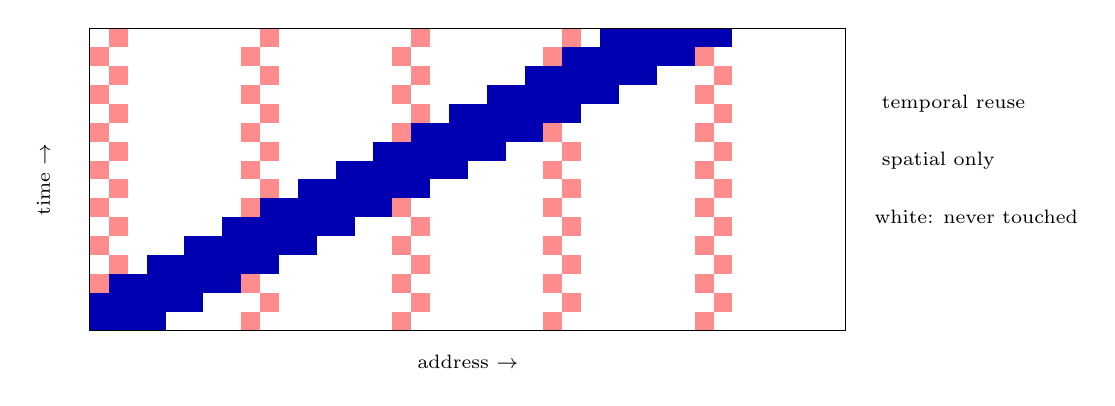
\begin{tikzpicture}[font=\scriptsize, x=2.4mm, y=2.4mm]
  % spatial-only speckle: addresses touched once near a used line
  \foreach \x in {0,...,39} \foreach \y in {0,...,15} {
    \pgfmathparse{mod(\x,8)==mod(\y,2) ? 1 : 0}
    \ifnum\pgfmathresult=1 \fill[red!45] (\x,\y) rectangle (\x+1,\y+1);\fi
  }
  % temporal reuse band on top: same region revisited
  \foreach \x in {0,...,39} \foreach \y in {0,...,15} {
    \pgfmathparse{abs(\x-2*\y)<4 ? 1 : 0}
    \ifnum\pgfmathresult=1 \fill[blue!70!black] (\x,\y) rectangle (\x+1,\y+1);\fi
  }
  \draw (0,0) rectangle (40,16);
  \node[anchor=west] at (41,12) {\textcolor{blue!70!black}{$\blacksquare$} temporal reuse};
  \node[anchor=west] at (41,9)  {\textcolor{red!45}{$\blacksquare$} spatial only};
  \node[anchor=west] at (41,6)  {white: never touched};
  \node[anchor=north] at (20,-0.8) {address $\to$};
  \node[rotate=90, anchor=south] at (-1.6,8) {time $\to$};
\end{tikzpicture}
\caption{The two kinds of locality, drawn as an address-$\times$-time
map. Spatial locality (red) is free: the line arrives anyway.
Temporal reuse (blue) is the one that actually turns into hits ---
a cache only helps if the same line is touched again before eviction.}
\label{fig:locality09}
\end{figure}
